\section{Facebook style notifications}

\subsection{Problem Summary}

\hspace{0.35cm} Many, different types of updates frequently happen in a course on Bodhitree. For example, some new videos may be added, quizzes may be published, exam marks might be uploaded etc. The user can only know about these updates by manually discovering them by visiting a concept page, checking for the published marksheets and so on.
\par There is a need to keep the users updated of what has been added to the course that they are enrolled into since they last checked the course contents. This will help the users to have a better grasp of the course contents by not missing out on any new additions that have been made to the course.

\subsection{Specifications}

\begin{enumerate}
	\item There must be a notifications button which should cover the following updates for a course:
	\begin{enumerate}
		\item Publishing a new concept
		\item Addition of new videos and documents
		\item Publishing new quizzes
		\item Uploading marksheet
		\item Addition of new threads in discussion forum
	\end{enumerate}
	\item The current number of notifications that have been pushed to the user must be displayed, which can be clicked to show more information.
	\item An expandable list should be present which lists the above updates and provides hyperlinks to them to enable easy navigation.
	\item The user must be able to clear the notifications, following which only those updates will be shown that are added after the user has cleared the notifications.
	\item The notifications must be categorised, and the number of notifications for each category must be shown to the users on the drop down list instead of showing all the notifications.
	\item Notifications must be course specific. When a user is on a particular course page, he should only see the notifications for that course.
\end{enumerate}

\subsection{System Design}

\hspace{0.35cm} The notifications system was designed using the push as well as the pull based mechanism. The course updates are pushed to the database and the user pull these updates whenever he logs into Bodhitree. The details of the system are as follows: 

\subsubsection{Storing the notifications (PUSH)}

\begin{enumerate}
	\item Two database tables are created to store the notifications and map the updates to them to the users for specific courses.
	\item The \textbf{Notice} table stores the notification data containing:
	\begin{enumerate}
		\item \textit{course} field: It stores foreign key to the course to which the notification belongs.
		\item \textit{notice\_data}: Stores the description of the notification.
		\item \textit{notice\_url}: Stores the hyperlink to the update displayed by the notification.
		\item \textit{notice\_date}: Stores the date and time on which the notification has been added. 
	\end{enumerate}
	\item The \textbf{ClearNotice} table which stores the user and the associated time on which he has cleared the notifications. The fields are:
	\begin{enumerate}
		\item \textit{user}: It is a one to one mapping to the current user.
		\item \textit{clear\_time}: It stores the time on which the current user has cleared the notifications.
	\end{enumerate}
	\item A function \textbf{add\_new\_notice()} is created which takes the arguments: \textit{data, courseid} and \textit{url}. This function can be called during any update that occurs in a course to push the desired notification into the database.
\end{enumerate}

\subsubsection{Retrieving the notifications (PULL)}

\begin{enumerate}
	\item An API \textbf{get\_notifications()} was created which fetches notifications for the current user by taking the courseid as an argument.
	\item A \textit{clear\_time} field is present which denotes the time on which a user has cleared the notifications previously. All the notifications that are present in the database for that course after that particular time (\textit{clear\_time}) are retrieved by the API.
	\item In case the user has not requested for the notifications earlier, then a \textit{clear\_time} value is added against his id which is the current time. This makes a user who is visiting a course for the first time to not see any notifications for that course.
	\item A sample JSON displaying the get notifications request is shown in figure \ref{fig:get_notifications}.
	\begin{figure}[h]
		\centering
		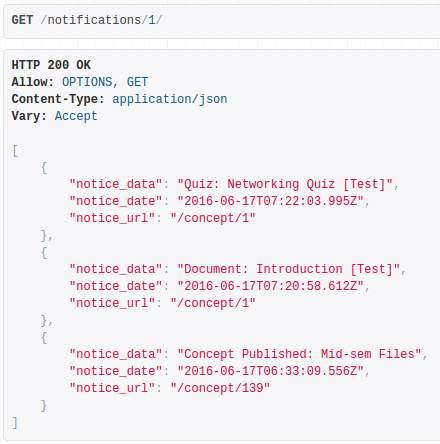
\includegraphics[width=0.7\linewidth]{./media/get_notifications}
		\caption{JSON showing the data retrieved through the GET notifications request}
		\label{fig:get_notifications}
	\end{figure}
\end{enumerate}

\subsubsection{Notifications UI}

\begin{enumerate}
	\item The UI consists of the notifications indicator, the drop down list of notifications, and the detailed notifications page, as shown in figure \ref{fig:notifications_ui}
	\item The notifications indicator is displayed as a leaf icon with a badge showing the number of pending notifications.
	\item Clicking on the indicator opens a drop down list which shows the notifications in a categorised way.
	\item There are two more buttons in the list to clear the notifications and see the detailed version which takes you to the detailed notifications page.
	\begin{figure}[h]
		\centering
		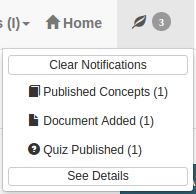
\includegraphics[width=0.3\linewidth]{./media/notifications_ui}
		\caption{Notifications indicator along with the drop down list}
		\label{fig:notifications_ui}
	\end{figure}
	\item The list shows the number of updates contained in each categories of notifications.
	\item In the detailed view, all the notifications are shown which are interactive. Clicking on these notifications takes you to the corresponding updates.
	\item The detailed notifications view is shown in figure \ref{fig:notifications_detailed}. Along with the interactive notifications, it also contains buttons to clear the notifications and to go on the previous page.
	\begin{figure}[h]
		\centering
		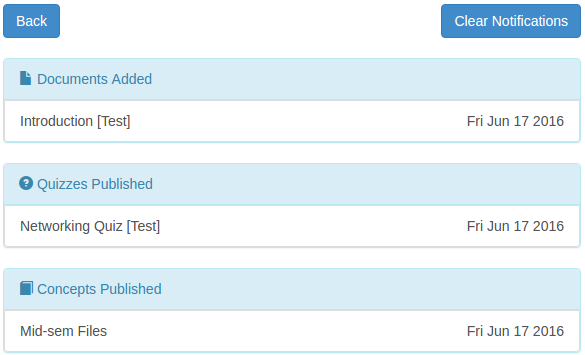
\includegraphics[width=0.7\linewidth]{./media/notifications_detailed}
		\caption{Detailed notifications view}
		\label{fig:notifications_detailed}
	\end{figure}
\end{enumerate}

\subsubsection{Categorizing the notifications}

\begin{enumerate}
	\item Currently, the notifications are categorized into 6 groups:
	\begin{enumerate}
		\item Video added
		\item Quiz added
		\item Document added
		\item Concept published
		\item Discussion forum updates
		\item Marks uploaded
	\end{enumerate}
	\item Figure \ref{fig:get_notifications} shows the data from the GET request. The grouping is done based on the \textit{``notice\_data''} field of each notification.
	\item The first 3 letters are matched (Example: \textit{`Con'}, \textit{`Vid'}, \textit{'Doc'}, etc.) and then these notifications are pushed into their respective categories.
	\item The hyperlink to the update is then added to an anchor tag  (\textit{\textless a href=...\textgreater}) and the interactive notification is then displayed on the detailed notification page.
\end{enumerate}

\subsubsection{Clearing the notifications}

\begin{enumerate}
	\item As already mentioned above, only those notifications that have their time greater than the time at which the current user has cleared the notifications will be fetched from the database.
	\item The user can choose to clear the notifications by clicking on the \textit{Clear Notifications} button which is present on the drop down list of notifications as well as on the detailed notifications view.
	\item On clicking on the clear button, the current time is added against the user's name in the \textit{clear\_time} field of the \textit{clearnotice} database table.
	\item When the users fetches the notifications again, the notifications previous to the clearing time will not be displayed.
\end{enumerate}